\documentclass[aps, pra, onecolumn, longbibliography]{revtex4-2}
\usepackage[utf8]{inputenc}
\usepackage[spanish]{babel}
\usepackage{float}
\usepackage{amsmath}
\usepackage{amsfonts}
\usepackage{amssymb}
\usepackage{graphicx}
\usepackage{hyperref}
\usepackage{braket}

\newcommand{\Tr}{\operatorname{Tr}}

\begin{document}
\title{Factor de forma espectral de un caminante 2D con moneda CUE(4)}
\date{30 de septiembre de 2026}
\maketitle

En estas notas calculamos el factor de forma espectral (SFF) de un caminante
cuántico en un billar, con una moneda $4\times4$ tomada del ensamble CUE. Damos
la predicción analítica, las derivaciones y la comparación con simulaciones.
Marcamos con \textbf{[supuesto]} los pasos que no se derivan, y con
\textbf{[estimado]} los que solo dan el orden de magnitud.

% ---------------------------------------------------------------------------
\section{Modelo}

El espacio de Hilbert es $\mathcal H=\mathcal H_p\otimes\mathcal H_c$, con
$\dim\mathcal H_c=4$ y $\dim\mathcal H_p=N$, el número de sitios del billar
$\Omega\subset\mathbb Z^2$. La dimensión total es $D=4N$. El operador de
evolución es
\begin{equation}
    U=S\,C,\qquad C=\mathbb 1_p\otimes M,\qquad M\in U(4).
\end{equation}
Las direcciones son $c_1,c_2,c_3,c_4$ = izquierda, arriba, derecha, abajo, con
desplazamientos $\delta_c$. Escribimos $\bar c$ para la dirección opuesta. El
shift es
\begin{equation}
    S\ket{x,c}=
    \begin{cases}
        \ket{x+\delta_c,c} & \text{si } x+\delta_c\in\Omega,\\
        \ket{x,\bar c} & \text{si } x+\delta_c\notin\Omega.
    \end{cases}
    \label{eq:S}
\end{equation}
$S$ es una matriz de permutación real. La moneda $M$ es \emph{la misma en todos
los sitios} y se toma con la medida de Haar en $U(4)$ (CUE). Los promedios
$\langle\cdot\rangle$ son sobre $M$; la geometría queda fija.

El SFF es
\begin{equation}
    K(t)=\left\langle\left|\Tr U^t\right|^2\right\rangle_M ,
    \qquad \tau=t/D .
\end{equation}

% ---------------------------------------------------------------------------
\section{Predicción analítica}

\subsection{No hay parte desconectada}
Si $M\to e^{i\varphi}M$, entonces $U\to e^{i\varphi}U$ y
$\Tr U^t\to e^{it\varphi}\Tr U^t$. La medida de Haar es invariante bajo este
cambio, así que
\begin{equation}
    \langle\Tr U^t\rangle=e^{it\varphi}\langle\Tr U^t\rangle
    \;\Rightarrow\;
    \langle\Tr U^t\rangle=0\quad(t\ge1).
\end{equation}
Por lo tanto $K(t)$ ya es el SFF conexo.

\subsection{Clase de simetría}
Sea $P$ el operador que invierte la dirección, $P\ket{x,c}=\ket{x,\bar c}$.
Es real, simétrico y cumple $P^2=\mathbb 1$.

\emph{Paso 1: $PSP=S^{-1}$.} En el interior,
$PSP\ket{x,c_1}=PS\ket{x,c_3}=P\ket{x+\hat e_x,c_3}=\ket{x+\hat e_x,c_1}
=S^{-1}\ket{x,c_1}$. En la frontera, si $x+\delta_c\notin\Omega$, entonces
$S\ket{x,c}=\ket{x,\bar c}$ y $S^{-1}\ket{x,\bar c}=\ket{x,c}$. Por otro lado,
$PSP\ket{x,\bar c}=PS\ket{x,c}=P\ket{x,\bar c}=\ket{x,c}$. Las demás
direcciones son iguales. Como $S$ es real, $S^{-1}=S^T$.

\emph{Paso 2: condición sobre la moneda.} Usamos la forma simetrizada
$U'=C^{1/2}SC^{1/2}$, que tiene el mismo espectro que $U$. Sea $T=PK$, donde
$K$ es la conjugación compleja. Entonces
\begin{equation}
    TU'T^{-1}=\bigl(P\,C^{1/2*}P\bigr)\,S^{-1}\,\bigl(P\,C^{1/2*}P\bigr).
\end{equation}
Esto es igual a $U'^{-1}=C^{-1/2}S^{-1}C^{-1/2}$ si $P M^{1/2*}P=M^{-1/2}$.
Al elevar al cuadrado queda $PM^*P=M^\dagger$, que es equivalente a
\begin{equation}
    PM=(PM)^T .
    \label{eq:TRS}
\end{equation}
Para la moneda de Grover (simétrica y conmuta con $P$) se cumple
\eqref{eq:TRS}. Para $M$ genérica de CUE no se cumple.

\textbf{[supuesto]} No probamos que no exista \emph{ningún} otro operador
antiunitario; solo revisamos $T=PK$ y sus composiciones con simetrías
geométricas. Si $g$ es una simetría de $\Omega$ que permuta las direcciones
con $\pi_g$, la simetría unitaria $G=g\otimes\pi_g$ conmuta con $S$. Conmuta
con $C$ solo si $\pi_g M\pi_g^T=M$, y $M$ genérica tampoco cumple esto.

\textbf{[supuesto]} La dinámica en el billar es caótica, como se pide.

Con estos dos supuestos, la clase esperada es CUE de dimensión $D=4N$.

\subsection{Rampa y meseta}
Para CUE de dimensión $D$ se tiene, de forma exacta,
\begin{equation}
    K(t)=\min(t,D)\quad(t\ge1),
    \qquad\text{o sea}\qquad
    \frac{K}{D}=\min(\tau,1).
    \label{eq:CUE}
\end{equation}
\textbf{[supuesto]} Si la densidad de eigenfases $\rho(\theta)$ no es plana
(normalizada a $\int\rho\,d\theta=D$) y el espectro es localmente CUE, entonces
\begin{equation}
    K(t)\simeq\bigl|\hat\rho(t)\bigr|^2
    +\int_0^{2\pi}\!d\theta\,\min\!\Bigl(\frac{t}{2\pi},\rho(\theta)\Bigr),
    \qquad \hat\rho(t)=\int d\theta\,\rho(\theta)e^{it\theta}.
    \label{eq:nonflat}
\end{equation}
El primer término no se cancela con el promedio: el cambio de fase global solo
multiplica $\hat\rho(t)$ por $e^{it\varphi}$. Después del unfolding se recupera
\eqref{eq:CUE}. La ec.~\eqref{eq:CUE} solo vale después de un tiempo de
Thouless $t_{\rm Th}$. Las secciones siguientes tratan los tiempos cortos.

% ---------------------------------------------------------------------------
\section{Tiempos cortos: resultados exactos y estimados}

\subsection{$t=1$ (exacto)}
Usando \eqref{eq:S},
$\bra{x,c}U\ket{x,c}=\sum_{c'}M_{c'c}\bra{x,c}S\ket{x,c'}$. El elemento de $S$
es distinto de cero solo si $c'=\bar c$ y la dirección $\bar c$ está bloqueada
en $x$. Definimos
$B_a=\#\{x\in\Omega:\;x+\delta_a\notin\Omega\}$, el número de sitios con la
dirección $a$ bloqueada. Entonces
\begin{equation}
    \Tr U=\sum_c B_{\bar c}\,M_{\bar c c}.
\end{equation}
Con $\langle M_{ij}M^*_{kl}\rangle=\delta_{ik}\delta_{jl}/4$,
\begin{equation}
    \boxed{K(1)=\frac14\sum_a B_a^2 .}
    \label{eq:K1}
\end{equation}
La predicción de RMT es $K(1)=1$. Aquí $K(1)$ crece como el perímetro al
cuadrado.

\subsection{Paridad: $t$ impar contra $t$ par (exacto)}
Un salto en el interior cambia la paridad de $x+y$; una reflexión en la
frontera no la cambia. Un camino cerrado de longitud $t$ con $n_r$ reflexiones
tiene $t-n_r$ saltos, y para cerrar se necesita que $t-n_r$ sea par. Si $t$ es
impar, $n_r$ es impar, así que todo camino que contribuye toca la frontera.
Por eso, para $t$ impar $\Tr U^t=O(\text{frontera})$, y para $t$ par
$\Tr U^t=O(N)$.

\subsection{$t=2$ (parte del bulto, exacta con Weingarten)}
Consideremos los caminos cerrados de longitud 2 sin reflexión. La moneda pasa
$c\to c'$, el caminante salta $\delta_{c'}$, la moneda pasa $c'\to c$ y el
caminante salta $\delta_c$. Para cerrar se necesita $c'=\bar c$. El número de
sitios donde esto es posible es $N-B_{\bar c}$. Entonces
\begin{equation}
    \Tr U^2\big|_{\rm bulto}
    =\sum_c (N-B_{\bar c})\,M_{\bar c c}M_{c\bar c}
    =s_{13}\,M_{13}M_{31}+s_{24}\,M_{24}M_{42},
\end{equation}
con $s_{13}=2N-B_1-B_3$ y $s_{24}=2N-B_2-B_4$. Para Haar en $U(d)$, con índices
distintos,
$\langle|M_{13}|^2|M_{31}|^2\rangle=\mathrm{Wg}(e,d)=1/(d^2-1)=1/15$. El
término cruzado se anula porque los índices de renglón $\{1,3\}$ y $\{2,4\}$ no
coinciden. Así,
\begin{equation}
    \boxed{K(2)\simeq\frac{s_{13}^2+s_{24}^2}{15}\;\approx\;\frac{8N^2}{15}.}
    \label{eq:K2}
\end{equation}
Faltan los caminos con dos reflexiones en el mismo sitio (esquinas). No los
calculamos.

\subsection{Decaimiento para $t$ par \textbf{[estimado]}}
Lejos de la frontera, $U$ es invariante ante traslaciones. En el espacio de
momentos queda $U(\mathbf k)=\Delta(\mathbf k)M$, con
$\Delta=\mathrm{diag}(e^{-ik_x},e^{ik_y},e^{ik_x},e^{-ik_y})$. El término de
Weyl es
\begin{equation}
    \Tr U^t\simeq N\!\int\!\frac{d^2k}{(2\pi)^2}\,\operatorname{tr}\bigl[(\Delta(\mathbf k)M)^t\bigr]
    =N\sum_{j=1}^{4}\int\!\frac{d^2k}{(2\pi)^2}\,e^{it\omega_j(\mathbf k)} .
\end{equation}
Con $\mathbf k\to\mathbf k+(\pi,\pi)$ se tiene $\Delta\to-\Delta$, así que la
integral se anula para $t$ impar. Esto es consistente con la regla de paridad.
Para $t$ par, la fase estacionaria en 2D da $O(1/t)$ por cada punto
estacionario no degenerado \textbf{[supuesto: sin puntos degenerados]}. Por lo
tanto
\begin{equation}
    K(t)\sim A\,\frac{N^2}{t^2}\qquad(t\ \text{par}).
\end{equation}
Este término es $|\hat\rho(t)|^2$ en \eqref{eq:nonflat}. Se cruza con la rampa
$t$ cuando $t^3\sim AN^2$, o sea $\tau^*\sim D^{-1/3}$, que tiende a cero para
billares grandes. Después del unfolding este término desaparece.

% ---------------------------------------------------------------------------
\section{Simulaciones}

Usamos dos billares de Sinaí en la red. El estadio \emph{simétrico} es un
cuadrado de $30\times30$ con un disco de radio 8 en el centro ($N=692$,
$D=2768$, $B_a=46$). El estadio \emph{asimétrico} es un rectángulo de
$31\times27$ con un disco de radio 7 centrado en $(18.3,11.1)$ ($N=683$,
$D=2732$, $B=(41,45,41,45)$).
\begin{itemize}
    \item \emph{Espectro completo:} 120 monedas CUE por geometría,
    diagonalización exacta y $K(t)$ para $1\le t<3D$. El unfolding usa la
    escalera de cada realización suavizada con una gaussiana de ancho
    $w=0.05$ en $\theta$.
    \item \emph{Tiempos cortos:} 6000 monedas por geometría. Se calcula
    $\Tr U^t$ con matrices dispersas para $t\le14$.
\end{itemize}
El código y los datos están en \texttt{code/}.

\subsection{Tiempos cortos: comparación con las fórmulas exactas}

\begin{table}[H]
\centering
\begin{tabular}{lcccc}
\hline\hline
 & \multicolumn{2}{c}{$K(1)/D$} & \multicolumn{2}{c}{$K(2)/D$}\\
 & ec.~\eqref{eq:K1} & numérico & ec.~\eqref{eq:K2} & numérico\\
\hline
Simétrico  & 0.764 & $0.778\pm0.010$ & 80.41 & $80.4\pm1.4$\\
Asimétrico & 0.678 & $0.691\pm0.009$ & 79.96 & $79.9\pm1.4$\\
\hline\hline
\end{tabular}
\caption{Valores exactos a $t=1,2$ comparados con la simulación (6000
realizaciones). La predicción de CUE sería $K/D=t/D\approx4\times10^{-4}$ y
$7\times10^{-4}$.}
\label{tab:short}
\end{table}

Para $t$ impar, $K/D$ se queda en $O(1)$ (entre 0.5 y 1.5). Para $t$ par es de
orden $10$--$10^2$. Esto confirma la regla de paridad. Para $t$ par entre 8 y
14, $K(t)\,t^2/D$ vale 1572, 1513, 1481 y 1451 (estadio simétrico). Es casi
constante, como pide el estimado $\propto t^{-2}$, aunque baja un poco. No
revisamos cómo escala con $N$.

\begin{figure}[H]
    \centering
    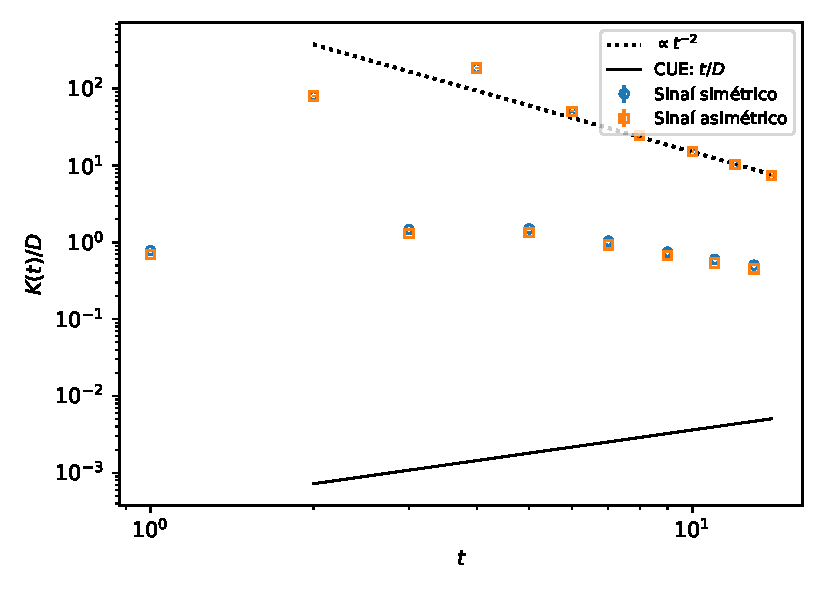
\includegraphics[width=0.55\textwidth]{Imgs/SFF_short.pdf}
    \caption{$K(t)/D$ exacto para $t\le14$ (6000 realizaciones). Los puntos
    altos son $t$ par y los bajos $t$ impar. La línea punteada es
    $\propto t^{-2}$; la continua, la rampa CUE $t/D$.}
    \label{fig:short}
\end{figure}

\subsection{Espectro completo}

\begin{table}[H]
\centering
\begin{tabular}{lc}
\hline\hline
 & $\langle r\rangle$\\
\hline
Simétrico  & $0.567\pm0.002$\\
Asimétrico & $0.582\pm0.001$\\
GUE / GOE / Poisson & 0.600 / 0.531 / 0.386\\
\hline\hline
\end{tabular}
\caption{Razón de espaciamientos consecutivos promedio.}
\end{table}

\begin{figure}[H]
    \centering
    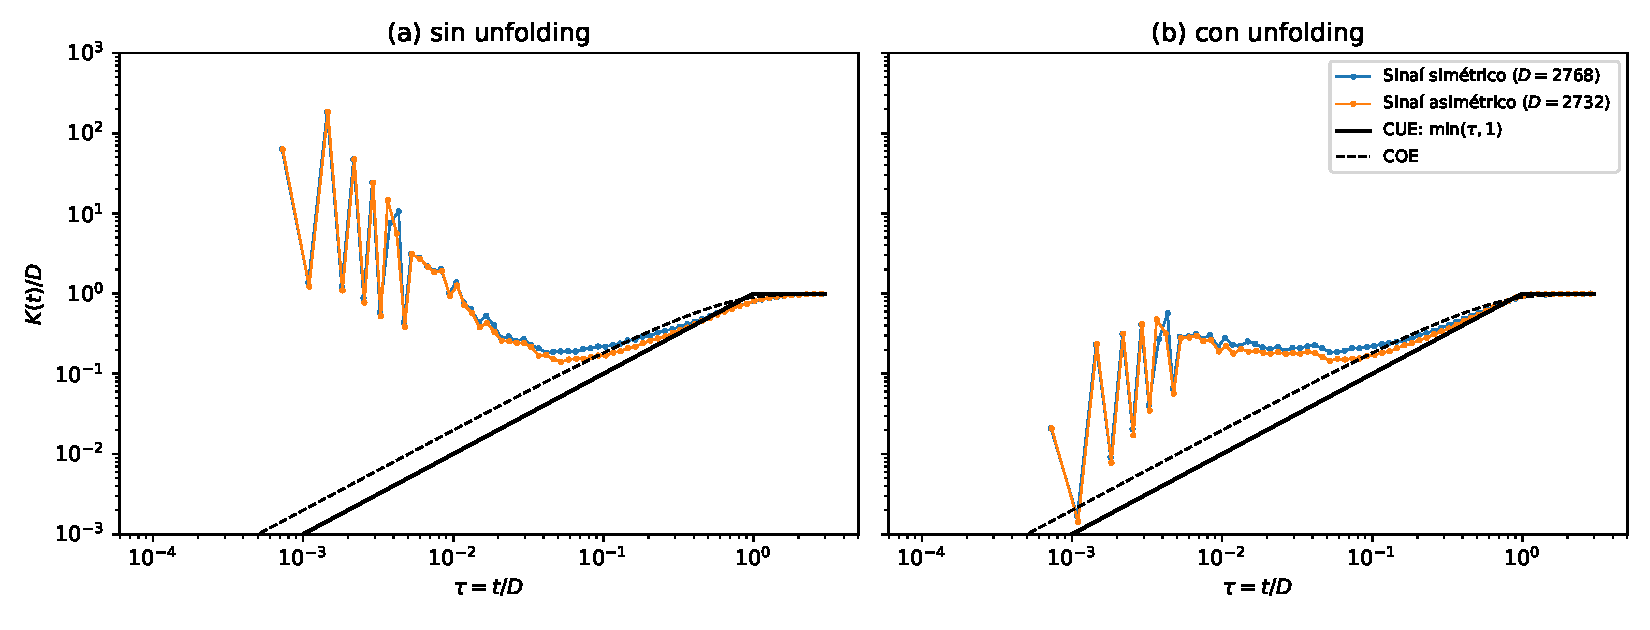
\includegraphics[width=\textwidth]{Imgs/SFF_CUEcoin.pdf}
    \caption{$K/D$ contra $\tau=t/D$, promediado en bins logarítmicos. (a) Sin
    unfolding. (b) Con unfolding. Línea continua: CUE, ec.~\eqref{eq:CUE}.
    Línea discontinua: COE.}
    \label{fig:sff}
\end{figure}

Lo que se observa en la figura~\ref{fig:sff}:
\begin{enumerate}
    \item \emph{Sin unfolding:} a $\tau\lesssim0.05$ hay un pico grande con la
    alternancia par/impar de la figura~\ref{fig:short}. Es el término
    $|\hat\rho(t)|^2$. La densidad de eigenfases de cada realización varía
    entre 0.23 y 2.15 veces la media.
    \item \emph{Con unfolding, estadio asimétrico:} para $\tau\gtrsim0.15$ los
    datos siguen la rampa CUE y la meseta $K/D=1$ en $\tau\ge1$.
    \item \emph{Con unfolding, estadio simétrico:} para $0.2\lesssim\tau<1$ los
    datos quedan entre COE y CUE. El valor $\langle r\rangle=0.567$ también
    está entre las dos clases.
    \item \emph{Con unfolding, ambos estadios:} para
    $0.005\lesssim\tau\lesssim0.1$ hay una meseta
    $K/D\approx0.15$--$0.2$, muy por encima de la rampa. El tiempo de Thouless
    efectivo es $t_{\rm Th}\approx0.15D\approx400$--$550$ pasos, mucho mayor
    que el tiempo de cruce balístico ($\sim30$ pasos).
\end{enumerate}

% ---------------------------------------------------------------------------
\section{Resumen y preguntas abiertas}

\begin{itemize}
    \item La predicción universal es $K/D=\min(\tau,1)$ (CUE, $D=4N$). Se
    cumple para $\tau\gtrsim0.15$ en el estadio sin simetrías geométricas.
    \item Los tiempos cortos no son universales porque la moneda es la misma en
    todos los sitios: promediar sobre $M$ no aleatoriza la parte de bulto. Los
    resultados exactos \eqref{eq:K1} y \eqref{eq:K2} coinciden con la
    simulación dentro del error.
    \item \textbf{Abierto:} por qué el estadio simétrico se acerca a COE, si
    \eqref{eq:TRS} no se cumple. Puede haber un antiunitario que combine $P$
    con una simetría geométrica del cuadrado, o puede ser un efecto de tamaño
    finito. No lo verificamos.
    \item \textbf{Abierto:} el origen de la meseta $K/D\approx0.2$ antes de
    $t_{\rm Th}$. Candidatos no verificados: órbitas tipo \emph{bouncing ball}
    del Sinaí, o estados con velocidad de grupo casi nula en la red.
    \item No corrimos otros tamaños, así que no sabemos cómo escalan
    $t_{\rm Th}$ ni la meseta con $N$.
\end{itemize}

\end{document}
